\documentclass[12pt]{article}
\usepackage{coursenote}
\newcommand\SSR{\text{SSR}}
\newcommand\SSE{\text{SSE}}

\begin{document}
\title{STAT 401 Chapter 16.1--16.6, 17.1--17.3}
\maketitle

\section{Single-factor ANOVA model (one-way ANOVA)}

\example Bread volume.

\example Drug dosage, page 677.

ANOVA models are linear regression models where
\begin{itemize}
\item either all predictors are qualitative, or
\item quantitative predictors are treated as qualitative,
    i.e.\@ cut into several levels.
\end{itemize}

Suppose the only factor has $r$ levels (i.e.\@ treatments).
Let $i$, $i=1,\dotsc,r$ denote treatment, and
$j$, $j=1,\dotsc,n_i$ denote individual observations (experimental
units) with treatment $i$, where $n_i$ is the number of observations
with treatment $i$.
The total sample size is $n_T = \sum_{i=1}^r n_i$.

If all $n_i$'s are equal, it's a \emph{balanced} design;
otherwise, \emph{unbalanced}.

The $j$th response in treatment $i$ is written
$Y_{ij}$.

\subsection{Model formulation: cell means model}

\[
Y_{ij} = \mu_i + \epsilon_{ij}
\]
The model has $r$ coefficients, $\mu_1,\dotsc,\mu_r$.
Interpretation:
the $j$th response of the $i$th treatment group
is a constant $\mu_i$, which is specific to the treatment,
plus a random fluctuation $\epsilon_{ij}$,
which is specific to this individual observation.
Naturally, $\mu_i$ is some kind of a mean value for the treatment $i$.

It's called a \emph{cell means} model:
each treatment group is a ``cell'' and we model the ``mean'' in the cell
by $\mu_i$.

\emph{Model assumptions}
\begin{enumerate}
\item $E(\epsilon_{ij}) = 0$. As a result, $E(Y_{ij}) = \mu_i$.
Therefore, $\mu_i$ is the expected response for treatment $i$.
\item $\var(\epsilon_{ij}) = \sigma^2$. Note by writing $\sigma^2$ without
any subscripts or modifiers involving $i$ or $j$, we mean the variance
is constant across $i$ and $j$.

Consequently, $\var(Y_{ij}) = \var(\epsilon_{ij}) = \sigma^2$ (because
$\mu_i$ is a constant).

\item The error terms are independent.
Consequently, the responses ($Y_{ij}$'s) are independent.

\item $\epsilon_{ij}$ has a normal distribution,
i.e.\@ $\epsilon_{ij} \overset{\text{iid}}{\sim} N(0, \sigma^2)$.
Consequently, $Y_{ij}$ is also normal:
$Y_{ij} \overset{\text{ind}}{\sim} N(\mu_i, \sigma^2)$.
(Note: $Y_{ij}$ are independent, but not iid. Their distributions
are not identical---they have different means.)
\end{enumerate}

\emph{Fixed effects} vs \emph{random effects} ANOVA models; page 685.
We deal with fixed effects models only.


\subsection{The ANOVA model is a linear model}

The ANOVA model is a linear model in which all the predictors are
qualitative.

In the cell-means formulation, we do not use an intercept.
As a result, we use $r$ indicators to encode the qualitative predictor
that has $r$ levels.
The coefficient for the $i$th indicator
(now written as $\mu_i$)
is simply the intercept of the model for the $i$th treatment level.

The coefficient vector is $\vec{\beta} = [\mu_1,\dotsc,\mu_r]'$
(without an intercept term).

The design matrix $\mat{X}$ is simple; see (16.6) on page 683.
It contains all 0's and 1's.
In each row there is exactly one instance of 1.

\alert
The cell-means formulation is \emph{equivalent} to a
``regular'' linear model with intercept and
$r-1$ indicators representing the qualitative predictor
that has $r$ treatments.
The effects of both formulations are the same:
each treatment gets its own mean (or intercept).
The model's performance in fitting data in both formulations
are exactly the same---after all both formulations
are the \emph{same model}. (See ``Computation''.)
Their difference is superficial; it's due to
the different ways of coding the factor.


\subsection{Fitting ANOVA model: the hefty way}

\emph{Dot notation}
A dot in the subscript means the index position taken by the dot is
aggregated over.

\begin{gather*}
Y_{i.} \equiv \sum_{j=1}^{n_i} Y_{ij},\quad
\overline{Y}_{i.} \equiv \frac{Y_{i.}}{n_i}\\
Y_{..} \equiv \sum_{i=1}^r \sum_{j=1}^{n_i} Y_{ij},\quad
\overline{Y}_{..} \equiv \frac{Y_{..}}{n_T}\\
\end{gather*}

\emph{LS estimation}:

\[
Q = \sum_{i=1}^r \sum_{j=1}^{n_i} (Y_{ij} - \mu_i)^2
\]

To find the $\mu_i$ that minimizes $Q$,
take derivative and set to zero:
\[
\frac{\diff Q}{\diff \mu_i}
= \frac{\diff\, \bigl(\sum_i\sum_j (Y_{ij} - \mu_i)^2\bigr)}{\diff \mu_i}
= \frac{\diff\, \bigl(\sum_{j=1}^{n_i} (Y_{ij} - \mu_i)^2\bigr)}{\diff \mu_i}
= -2\sum_j (Y_{ij} - \mu_i)
= 2n_i\mu_i - 2Y_{i.}
= 0
\]
\[
\Longrightarrow
\hat{\mu}_i = \overline{Y}_{i.}
\]
We see indeed the estimation of $\mu_i$
is just the mean response of the treatment $i$.
(Maximum likelihood estimation is the same.)

\emph{Fitted value}:
for $Y_{ij}$, the fitted value is $\hat{\mu}_i$,
that is, $\overline{y}_{i.}$, the mean response of its treatment group.

\emph{Residual}:
$e_{ij} = Y_{ij} - \hat{Y}_{ij} = Y_{ij} - \overline{Y}_{i.}$.

Note: residuals of the same treatment group sum to zero:
$\sum_{j=1}^{n_i} e_{ij} = 0$.
(Of course, the sum of all residuals is also zero.)


\subsection{Fitting ANOVA model: the smart way}

\[
\vec{\hat{\mu}}
= \bigl(\mat{X}^T\mat{X}\bigr)^{-1} \mat{X}^T \vec{Y}
\]
Noticing the special structure of the design matrix $\mat{X}$,
$\mat{X}^T\mat{X}$ is a diagonal matrix with
$n_1,\dotsc,n_r$ on the diagonal.
Hence $\bigl(\mat{X}^T\mat{X}\bigr)^{-1}$ is diagonal with
$\frac{1}{n_1},\dotsc,\frac{1}{n_r}$ on the diagonal.
$\mat{X}^T\vec{Y}$ is the vector with elements
$Y_{1.},\dotsc,Y_{r.}$.
Then you get the same estimates of $\mu_i$ as above.


\section{ANOVA model vs regression model}

\begin{itemize}
\item If all predictors are qualitative,
regression and ANOVA models are equivalent.
\item The emphasis of an ANOVA model is whether there are ``treatment
effects'', i.e.\@ whether the $\mu_i$'s are not all equal.
This will be examined via analysis of variance and $F$ test.

\item When there are multiple factors, additional emphasis of ANOVA
includes interactions between the factors, and the contributions
of factors to SS.

\item The fundamental difference between a quantitative predictor and a
qualitative predictor is the former has a meaning of ``order and
distance'', whereas for the latter different values are just
``different'' and no more.

Suppose our dataset $(X, Y)$ is
$(1,y_1)$, $(2,y_2)$, $(3,y_3)$,..., $(9, y_9)$.
Suppose we square $X$, then the data become
$(1, y_1)$, $(4, y_2)$, $(9, y_3)$,..., $(81, y_9)$.
If you make a plot, we see the relation (curve) changes, because the
squaring changes the distances between the $X$ values.

This is why in a regression model with quantitative predictors we need
to worry about the ``form'' of the relation.

If $X$ is qualitative, say with values 'A', 'B', 'C',....
You transform $X$, they're still ``just different'' (so transformation
makes no sense). Therefore with qualitative predictors, there are no
different ``forms'' of relations; the question is just whether $Y$ is
systematically ``different'' for different values (levels) of $X$.

In a regression model, an important task is to find
$E(Y) = f(X)$, the correct ``form'' of the function $f$.
\end{itemize}

\section{Analysis of variance}

Let's call the only qualitative predictor $X$
and denote the constant 1 by $X_0$ as before.

The cell means model is
\[
Y = \vec{\mu}^T \vec{x} + \epsilon
\]
where $\vec{x}$ is the vector of indicators that
encode the qualitative predictor $X$.

As before, we define
\[
\text{SST}
\overset{\text{def}}{=} \sum_i\sum_j Y_{ij}^2
\]
\[
\SSR
\overset{\text{def}}{=} \sum_i\sum_j \hat{Y}_{ij}^2
= \sum_i n_i \overline{Y}_{i.}^2
\]
\[
\SSE
\overset{\text{def}}{=} \sum_i\sum_j (Y_{ij} - \hat{Y}_{ij})^2
= \sum_i\sum_j (Y_{ij} - \overline{Y}_{i.})^2
\]
and we have
\begin{equation}\label{eq:SST=SSR+SSE}
\text{SST} = \SSR + \SSE
\end{equation}

\exercise
Verify $\text{SST} = \SSR + \SSE$ using
the definitions above.
(In principle, there is no need to ``verify'' this relation
because we have proved it in the linear model lectures
and here is just a linear model.)

A main concern in this model is whether there is ``factor effect'',
that is, whether the cell means (for different factor levels, or
treatments) are indeed different.
To test this, we'll need to compare with the model in which
there is no factor effect, and that is the ``pure intercept'' model:
\[
Y = \mu_0 + \epsilon
\]
In this context,
\emph{the cell mean model is the ``full'' model whereas
the pure intercept model is the ``reduced'' model.}

\alert
We have commented earlier that
the full model (the cell-means model) is equivalent to a model
containing intercept and $r-1$ indicators.
In light of this equivalence,
the cell-means model is indeed an \emph{expansion} of the pure-intercept model.
It is backed by this fact
that we call the cell-means model and the
pure-intercept model a pair of ``full'' and ``reduced'' models.

We'll be interested in $\SSR(X)$
(this is the $\SSR$ defined above),
$\SSR(X_0)$, $\SSR(X \given X_0)$,
and $\SSE(X_0)$, $\SSE(X)$ (this is the $\SSE$ defined above).

Because $\hat{\mu}_0 = \overline{Y}_{..}$, we see
\[
\SSE(X_0) = \sum_i\sum_j (Y_{ij} - \overline{Y}_{..})^2
\]
Then the \emph{extra contribution to SS by the factor effect}
is
$\SSE_{\text{reduced}} - \SSE_{\text{full}}$, that is,
\[\begin{split}
\SSE(X_0) - \SSE(X)
&= \sum_i\sum_j (Y_{ij} - \overline{Y}_{..})^2
  -
  \sum_i\sum_j (Y_{ij} - \overline{Y}_{i.})^2
\\
&= \sum_i\sum_j (2Y_{ij} - \overline{Y}_{..} - \overline{Y}_{i.})
    (\overline{Y}_{i.} - \overline{Y}_{..})
\\
&= \sum_i (\overline{Y}_{i.} - \overline{Y}_{..})
    (2n_i\overline{Y}_{i.} - n_i\overline{Y}_{..} -
        n_i\overline{Y}_{i.})
\\
&= \sum_i (\overline{Y}_{i.} - \overline{Y}_{..})
    (n_i\overline{Y}_{i.} - n_i\overline{Y}_{..})
\\
&= \sum_i n_i (\overline{Y}_{i.} - \overline{Y}_{..})^2
\\
&= \sum_i \sum_j (\overline{Y}_{i.} - \overline{Y}_{..})^2
\end{split}
\]
We call $\sum_i\sum_j (Y_{ij} - \overline{Y}_{i.})^2$
``within-treatment'' variation, and
$\sum_i\sum_j (\overline{Y}_{i.} - \overline{Y}_{..})^2$
``between-treatment'' variation.
The former is the sum of squares due to random fluctuations
of individual observations around their corresponding treatment means
(i.e.\@ noise);
the latter is the sum of squares due to fluctuations
of the treatment means about the grand mean (i.e.\@ treatment effects).
The extra SSR due to $X$ is an account of the
``between-treatment variation''.
The relation above also suggests
\begin{equation}\label{eq:SSTO}
\begin{split}
\SSE(X_0)
&= \SSE(X) + \sum_i\sum_j (\overline{Y}_{i.} - \overline{Y}_{..})^2
\\
&=
  (\text{within-treatment variation})
  \;+\;
  (\text{between-treatment variation})
\end{split}
\end{equation}
(This is relation (16.30) on page~691.)
KNNL calls
$\sum_i\sum_j (Y_{ij} - \overline{Y}_{..})^2$
the ``total variation'' and denotes it by
$\text{SSTO}$.
We call it $\SSE(X_0)$ ($\SSE$ of the reduced model),
to be consistent with the linear model lectures.

\alert
$\text{SSE}(X)$ is the SSE of the ``full'' model.
There is some notational confusion here.
In the style of the previous linear model chapters,
this would have been written as $\text{SSE}(X_0, X)$
because the model \emph{in effect} contains intercept
as well as the only qualitative predictor.
The intercept does not show up because of the particular choice
in coding the factor by indicators.
In effect, the full model introduces the predictor $X$
to the ``pure-intercept'' model.
In the ``linear-model'' way this would have been done by
using $r-1$ indicators, but here $r$ indicators are used,
which kick the intercept out of the model formulation.


\subsection*{Degrees of freedom}

In relation~(\ref{eq:SST=SSR+SSE}), the df's are
$n_T$, $r$, $n_T - r$.

In relation~(\ref{eq:SSTO}), the df's are
$n_T - 1$, $n_T - r$, $r-1$.


\subsection*{ANOVA table}

Table 16.3, page 694.

However, since we are using somewhat different notation,
you only need to understand this example table but do not need to follow
it.

We'll see more of this in \verb+R+ output.

\section{$F$ tests for equality of factor level means}

The basic test for an ANOVA model is about
$\mu_1=\dotsb=\mu_r$, that is, treatments have the same mean
(i.e.\@ no treatment effect).

Hypotheses:\\[3pt]
$H_0$: $\mu_1 = \dotsb = \mu_r$\\
$H_a$: $\mu_1, \dotsc, \mu_r$ not all equal\\

$H_0$ corresponds to the reduced model (the pure intercept model),
whereas
$H_a$ corresponds to the full model (the cell means model).

The test statistic is, of course, the old idea:
\[\begin{split}
F^*
&=
\frac{\SSE_{\text{reduced}} - \SSE_{\text{full}}}
    {\#\{\text{coefs in full model}\}
     - \#\{\text{coefs in reduced model}\}}
\biggm/
\frac{\SSE_{\text{full}}}
    {n_T - \#\{\text{coefs in full model}\}}
\\
&\sim F_{r-1,\, n_T - r}
\end{split}
\]

\alert
$\text{SSE}_{\text{reduced}}$ is
$\text{SSE}(X_0)$,
i.e.\@ $\sum_i\sum_j (Y_{ij} - \overline{Y}_{..})^2$.
$\text{SSE}_{\text{full}}$ is
$\text{SSE}(X)$,
i.e.\@ $\sum_i\sum_j (Y_{ij} - \overline{Y}_{i.})^2$.

Critical value: $F(1-\alpha; r-1, n_T - r)$

Decision rule: $H_a$ if $F^* > F(1-\alpha; r-1, n_T - r)$; $H_0$
otherwise.

$P$-value: $1 - \operatorname{cdf}(F^*; r-1, n_T-r)$.

\example
page 699.


\section{Inferences for a single treatment mean}

\example
Kenton Food Company (p.~685): potential influence of
packaging design on sales.

\example
Rust inhibitors (p.~734): 4 brands. $Y$ is effectiveness of the rust
inhibitor.


As before, ``inference'' means either
(1) point estimation and construction of confidence interval (CI),
or (2) test of statistical hypothesis.
Solution to both problems rely on the same tool:
sampling distribution of a chosen statistic of the data.

Of concern is the cell means model
\[
Y_{ij} = \mu_i + \epsilon_{ij}
\]
and the $r$ treatment means $\mu_1, \dotsc, \mu_r$.

Recall the model assumption:
\[
\epsilon_{ij} \overset{\text{iid}}{\sim} N(0, \sigma^2)
,\text{ or equivalently, }
Y_{ij} \overset{\text{ind}}{\sim} N(\mu_i, \sigma^2)
\]

The LS estimators for the model parameters are
\[
\hat{\mu}_i = \overline{Y_{i.}}
\]
\[
S^2
= (n_T-r)^{-1}\sum_i\sum_j (Y_{ij} - \hat{Y}_{ij})^2
= (n_T-r)^{-1}\sum_i\sum_j (Y_{ij} - \overline{Y_{i.}})^2
\]
$S^2$ is also called MSE.
All these estimators are unbiased
(if the model assumptions are satisfied).


\emph{What is the sampling distribution of $\hat{\mu}_i$?}

Note it is the mean of a random sample (of size $n_i$)
from the distribution $N(\mu_i, \sigma^2)$, hence
\[
\hat{\mu}_i \sim N(\mu_i, \sigma^2/n_i)
\]
Replacing $\sigma^2$ by its estimator $S^2$, we have
\[
\frac{\hat{\mu}_i - \mu_i}{\sqrt{S^2/n_i}} \sim t(n_T - r)
\]
Note: the df of the $t$ distribution is the df of $S^2$,
which is estimated using the entire dataset,
not only the data from the $i$th cell.

CI and tests for $\mu_i$ (the unknown, true parameter value) is based on
this sampling distribution.

$100(1-\alpha)\%$ CI:
\[
\overline{y}_{i.} \pm t(1-\alpha/2; n_T-r) \sqrt{s^2/n_i}
\]

Test for $H_0: \mu_i = c$ vs $H_a: \mu_i \ne c$:
reject if
\[
\biggl|\frac{\overline{y}_{i.} - c}{\sqrt{s^2/n_i}}\biggr|
> t(1-\alpha/2; n_T - r)
\]

% Recall the \emph{equivalence between CI and two-sided test}
% (using the same $\alpha$ level):
% if the CI contains the hypothesized value, conclude $H_0$;
% otherwise, reject.

\example Page 738.

\section{Inferences for linear combinations of treatment means}

Suppose we are interested in a linear combination of the treatment
means:
\[
L = \sum_{i=1}^r c_i \,\mu_i
\]
A point estimator for $L$ is naturally
\[
\hat{L}
= \sum_{i=1}^r c_i \,\hat{\mu}_i
= \sum_{i=1}^r c_i \,\overline{Y}_{i.}
\]
(In fact this is the best estimator for $L$ in a certain sense.)

\emph{What is the sampling distribution of $\hat{L}$?}

$\hat{L}$ is a linear combination of $\hat{\mu}_i$'s,
each of which is normal; in addition, $\hat{\mu}_i$ and $\hat{\mu}_j$
(where $i\ne j$) are independent. Therefore
\[
\hat{L} \sim N\Bigl(
    \sum_i c_i \,\mu_i,\;
    \sigma^2\sum_i c_i^2/n_i
    \Bigr)
\]
Consequently,
\[
\frac{\sum_i c_i\,\overline{Y}_{i.} - \sum_i c_i \,\mu_i}{
    \sqrt{S^2\sum_i c_i^2/n_i}}
\sim t(n_T - r)
\]
or
\[
\frac{\hat{L} - L}{\sqrt{S^2\sum_i c_i^2/n_i}}
\sim t(n_T - r)
\]

Inferences and tests about $L$ are based on this distribution.

A single treatment mean is apparently a special case of $L$.
Two other special cases follow.

\alert
Whare are $\hat{\mu}_i$ and $\hat{\mu}_j$, $i\ne j$,
independent?
Because $\hat{\mu}_i = \overline{Y}_{i.}$,
$\hat{\mu}_j = \overline{Y}_{j.}$,
and the observations in the two cells are independent.
This situation differs from that of, say,
$\hat\beta_i$ and $\hat\beta_j$ in a ``regular'' linear model,
in which both $\hat\beta_i$ and $\hat\beta_j$
are estimated from the entire set of $Y$'s and therefore
are usually dependent.

\subsection*{Inferences for difference between two treatment means}

Suppose we're interested in $\mu_i - \mu_j$ (where $1 \le i < j \le r$).
Inferences and tests are based on the following sampling distribution:
\[
\frac{(\overline{Y}_{i.} - \overline{Y}_{j.}) - (\mu_i - \mu_j)}
    {\sqrt{S^2\bigl(\frac{1}{n_i} + \frac{1}{n_j}\bigr)}}
\sim t(n_T - r)
\]

\example
Page 740.

This situation is a special case of the next.

\subsection*{Inferences for \emph{contrast} of treatment means}

If the coefficients $c_i$ sum to 0,
then $L$ is called a ``contrast''.

Examples of contrasts: page 741--742.

\example
Page 743.

\section{Computation}

\textbf{1}

How do we ``randomly assign'' treatments to experimental units?

Suppose we have 6 experimental units and 3 treatments,
and the 6 units show up in some sort of ``natural'' order.
If we take the first two for treatment 1,
the second two for treatment 2,
and the last two for treatment 3,
there could be some factor some has come along with
the natural order of the units, which will affect the result.
We need to randomize the order of the experimental units.
After that we can take regular blocks of the units
and assign treatments to them.
So the key is to \emph{randomly re-order} the units.

The \verb+R+ function \verb+sample(n)+
generates a \emph{permutation},
i.e.\@ random ordering, of the numbers 1,..., $n$.
\begin{verbatim}
> sample(6)
[1] 3 6 4 5 1 2
\end{verbatim}
Then we can take the
3rd and 6th units for treatment 1,
the 4th and 5th units for treatment 2,
and the 1st and 2nd units for treatment 3.


\textbf{2}

We use the SENIC dataset in Appendix C.

\begin{verbatim}
> data <- read.table('senic.txt', header = FALSE)
> print(names(data))
 [1] "V1"  "V2"  "V3"  "V4"  "V5"  "V6"  "V7"  "V8"  "V9"  "V10" "V11" "V12"
> data <- data[, c(3, 4, 9)]
> names(data) <- c('age', 'risk', 'region')
> 
> # 'region' is a numerical now, noticing
> # its values are 1, 2, 3, 4.
> # Convert it to categorical.
> data$region <- as.factor(data$region)
> print(is.factor(data$region))
[1] TRUE
> print(class(data$region))
[1] "factor"
> 
> # Make a plot.
> pdf(file = 'part16-a.pdf', width = 7, height = 5)
> plot(x = data$region, y = data$risk, xlab = 'region', ylab = 'risk')
> dev.off()
X11cairo 
       2 
>     # Whoops! Not what you hoped for!
>     # Since 'x' is of 'factor' type,
>     # R does not think a numerical scale makes sense to it.
>     # R makes a boxplots of all 'y' values with a common level
>     # of the factor 'x'. This plot actually IS quite informative.
> 
> # To make something similar to  Figure 16.3, page 686:
> pdf(file = 'part16-b.pdf', width = 7, height = 5)
> plot(x = as.numeric(data$region), y = data$risk, xlab = 'region', ylab = 'risk')
> dev.off()
X11cairo 
       2 
\end{verbatim}

\begin{center}
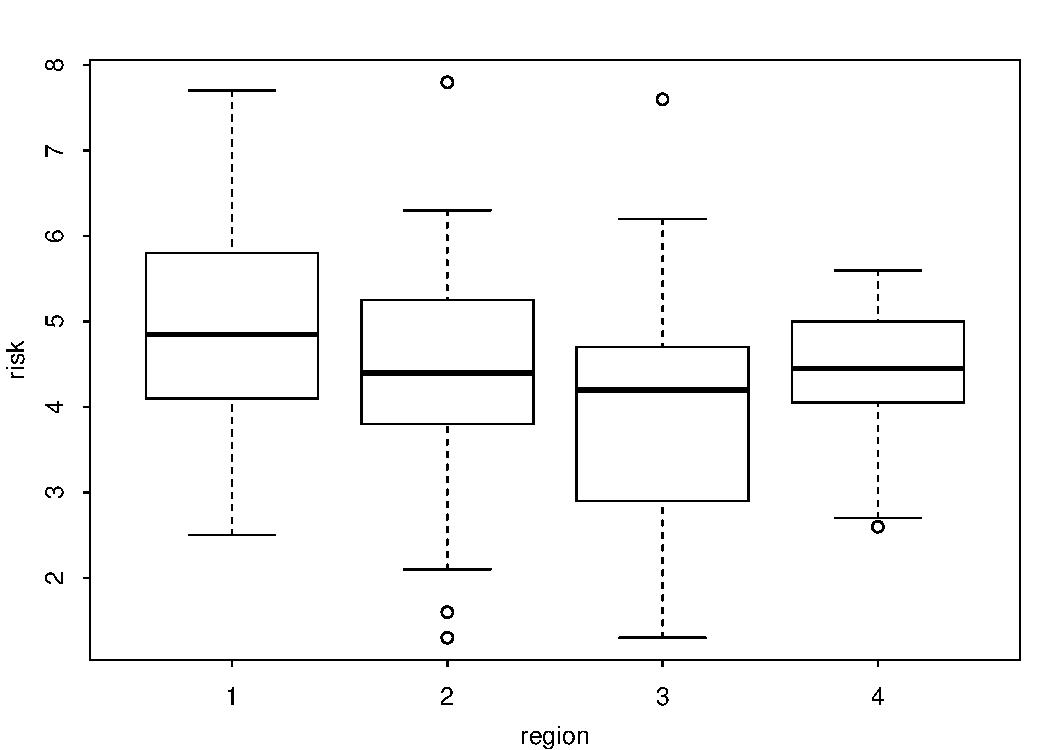
\includegraphics{part16-a.pdf}
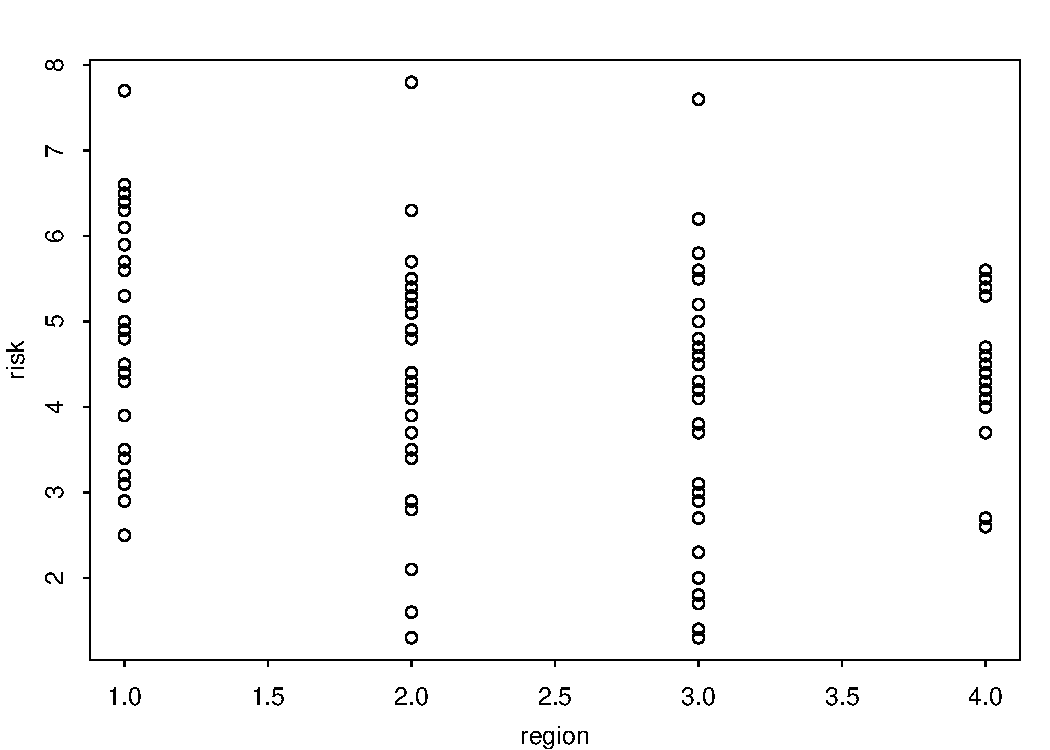
\includegraphics{part16-b.pdf}
\end{center}

\begin{verbatim}
> # Let's fit a linear model and take a look.
> lmfit <- lm(risk ~ region, data)
> print(lmfit)

Call:
lm(formula = risk ~ region, data = data)

Coefficients:
(Intercept)      region2      region3      region4  
     4.8607      -0.4670      -0.9337      -0.4795  

> print(summary(lmfit))

Call:
lm(formula = risk ~ region, data = data)

Residuals:
     Min       1Q   Median       3Q      Max 
-3.09375 -0.82703  0.03929  0.83929  3.67297 

Coefficients:
            Estimate Std. Error t value Pr(>|t|)    
(Intercept)   4.8607     0.2478  19.617  < 2e-16 ***
region2      -0.4670     0.3393  -1.376  0.17155    
region3      -0.9337     0.3284  -2.843  0.00534 ** 
region4      -0.4795     0.4109  -1.167  0.24582    
---
Signif. codes:  0 ‘***’ 0.001 ‘**’ 0.01 ‘*’ 0.05 ‘.’ 0.1 ‘ ’ 1 

Residual standard error: 1.311 on 109 degrees of freedom
Multiple R-squared: 0.06951,	Adjusted R-squared: 0.0439 
F-statistic: 2.714 on 3 and 109 DF,  p-value: 0.04839 

>     # Nothing we didn't see before.
\end{verbatim}

Note the intercept is included by default,
and 3 indicators are used to code the 4-level factor \verb+region+.
This is the usual linear model.

The cell-means formulation does not use intercept.
So let's refit.

\begin{verbatim}
> myfit <- lm(risk ~ -1 + region, data)
> print(myfit)

Call:
lm(formula = risk ~ -1 + region, data = data)

Coefficients:
region1  region2  region3  region4  
  4.861    4.394    3.927    4.381  

> print(summary(myfit))

Call:
lm(formula = risk ~ -1 + region, data = data)

Residuals:
     Min       1Q   Median       3Q      Max 
-3.09375 -0.82703  0.03929  0.83929  3.67297 

Coefficients:
        Estimate Std. Error t value Pr(>|t|)    
region1   4.8607     0.2478   19.62   <2e-16 ***
region2   4.3937     0.2318   18.96   <2e-16 ***
region3   3.9270     0.2156   18.22   <2e-16 ***
region4   4.3812     0.3278   13.37   <2e-16 ***
---
Signif. codes:  0 ‘***’ 0.001 ‘**’ 0.01 ‘*’ 0.05 ‘.’ 0.1 ‘ ’ 1 

Residual standard error: 1.311 on 109 degrees of freedom
Multiple R-squared: 0.9201,	Adjusted R-squared: 0.9171 
F-statistic: 313.7 on 4 and 109 DF,  p-value: < 2.2e-16 
\end{verbatim}

Carefully compare the printouts of \verb+lmfit+ and \verb+myfit+.

Because of the coding adopted in \verb+lmfit+,
the \verb+(Intercept)+ in \verb+lmfit+ is equal to the
\verb+region1+ in \verb+myfit+.
The \verb/(Intercept) + region2/ in \verb+lmfit+
is equal to the \verb+region2+ in \verb+myfit+.
And so on.

Also note the ``Residual standard error'' of the two models:
both are 1.311. The performance of fitting the data is equal,
because the two models are equivalent.

So far we've been fitting a regular linear model.
Since we know the predictors are all qualitative,
hence it is a ANOVA model, it is more natural to do that
directly the ``ANOVA way'', using \verb+aov+.

\begin{verbatim}

> aovfit <- aov(risk ~ region, data)
> print(aovfit)
Call:
   aov(formula = risk ~ region, data = data)

Terms:
                   region Residuals
Sum of Squares   13.99694 187.38288
Deg. of Freedom         3       109

Residual standard error: 1.311148 
Estimated effects may be unbalanced
> aovsummary <- summary(aovfit)
> print(aovsummary)
             Df  Sum Sq Mean Sq F value  Pr(>F)  
region        3  13.997  4.6656   2.714 0.04839 *
Residuals   109 187.383  1.7191                  
---
Signif. codes:  0 ‘***’ 0.001 ‘**’ 0.01 ‘*’ 0.05 ‘.’ 0.1 ‘ ’ 1 
\end{verbatim}

The table above is the ANOVA table that we pretty much
can copy and use directly for testing
$H_0: \mu_1=\mu_2=\mu_3=\mu_4$.

Look at the \verb+region+ row:
\verb+Df+ is 3 instead of 4.
This row shows the \emph{extra} SSR and MSR
of the predictor ``region'' on top
of an intercept.

Look at the \verb+Residuals+ row:
the \verb+Df+ is the same as that
in models \verb+lmfit+ and \verb+myfit+.
(Read the line\\
\verb+Residual standard error: 1.311 on 109 degrees of freedom+
in the output of \verb+summary+.)

Also note the MSE on the second row: 1.7191.
This is $s^2$, and is equal to $1.311^2$,
the square of $s$, which has been shown
in the \verb+summary+ of \verb+lmfit+ and \verb+myfit+.
So it's the same MSE.
The models \verb+lmfit+, \verb+myfit+, and \verb+aovfit+
are all equivalent.

The $F$ test in the table above is testing whether
the predictor \verb+region+ is significant,
compared to using intercept alone.
This is exact the test we need for ANOVA.

Finally, also note the last line of the output of
\verb+summary(lmfit)+.
It reports the result of a $F$ test, and it is the same result as that
in the table above, because it's the same test.
(In contrast,
\verb+summary(myfit)+ reports the result of a different test:
testing the significance of \verb+region+
compared with the model $Y = 0 + \epsilon$.
That is NOT the test we want.)

If all this looks confusing, perhaps the following
somewhat brute force procedure is better.

\begin{verbatim}
> fit.x <- lm(risk ~ -1 + region, data)
> fit.0 <- lm(risk ~ 1, data)
> sse.x <- deviance(fit.x)
> sse.0 <- deviance(fit.0)
> df.x <- length(coef(fit.x))  # 4
> df.0 <- 1
> df.ssr <- df.x - df.0
> df.sse <- nrow(data) - df.x
> ssr <- sse.0 - sse.x            # extra SSR
> msr <- ssr / df.ssr
> mse <- sse.x / df.sse
> f.star <- msr / mse
> f.crit <- qf(.95, df.ssr, df.sse)
> p.val <- 1 - pf(f.star, df.ssr, df.sse)
> print(c(df.ssr = df.ssr, df.sse = df.sse))
df.ssr df.sse
     3    109
> print(c(
+     ssr = ssr, sse = sse.x,
+     msr = msr, mse = mse,
+     f.star = f.star, f.crit = f.crit, p.value = p.val)
+     )
         ssr          sse          msr          mse       f.star       f.crit 
 13.99693932 187.38288369   4.66564644   1.71910902   2.71399101   2.68790809 
     p.value 
  0.04838638 
\end{verbatim}

Compare this result with that contained in
\verb+aovsummary+.

If you need to make inferences about individual treatment effects,
you need the estimate and standard error of each coefficient.
In that case you need to use the \verb+Coefficients+ block
of the output of \verb+summary(myfit)+,
because the coefficients in \verb+myfit+ are those treatment
means directly.


\end{document}
